\section{The Semantic Web}
\label{sec:semweb}

\subsection{A Quick History of the Web}

The idea of hypertext was at the basis of many of the developments of the Web. It was invented simultaneously in the 1960s by Engelbart and Nelson (see Section \ref{sec:visionaries} for more details) \cite{Engelbart1962,Engelbart1968,Nelson1965}. ``Enquire'' was created by \cite{BernersLee2000} at CERN twenty years later, in the early 1980s, and it was the first PIM system to use hypertext .

So far, the systems following the idea of hypertext, including Enquire, were limited to work with information from a single computer. Starting from 1984, Berners-Lee started to extend the system, to enable it to point to documents from other machines, using the existing Internet infrastructure, developed in the 1970s partly by the old hypertext community. Based on this extension, he proposed a system called ``Mesh'' \cite{BernersLee1989}, which incorporated technologies that have developed into today's Web: \emph{HyperText Markup Language} (HTML), \emph{HyperText Transfer Protocol} (HTTP) and \emph{Universal Resource Identifiers} (URIs). It was at CERN than Berners-Lee developed the first applications to use these technologies: the first Web browser and the first Web server. The ``Mesh'' was not a success when it was first created, but it was an open and distributed architecture, features that allowed others to develop their own browsers and publish their own documents. 

In Berners-Lee's implementation, Web documents were both readable and editable, but the editing functionality was ignored by the other browser implementations. Editing was both a very difficult task, and one that was not considered as important. Mosaic (1993) was the first widely available browser, which made the ``Web'' gain more and more popularity. The number of Web servers also grew, and so did the number of pages published.

\subsection{Semantic Web Technologies}

The World Wide Web \cite{BernersLee1994} allowed people to publish information easily. It provided read-only access to an immense quantity of information, which grew exponentially, as the technology evolved, and as having access to a faster and more reliable Internet connection became wide-spread. With the Semantic Web we move on from a Web of documents understood by humans to a Web of machine understandable information  \cite{BernersLee2001}. But this was not something new: most of the ideas we now attribute to the Semantic Web --- typed links and nodes --- were in fact present in the initial proposal of the Mesh, but they were omitted in favour of simplicity.

Thus, the goal of the Semantic Web is to add (machine understandable) meaning to the huge repository of connected information that is the Web. To accomplish this, the Semantic Web uses the same infrastructure and standards as the Web, along with additional technologies, which make up the ``Semantic Web layer cake''\footnote{\url{http://www.w3.org/2007/03/layerCake.svg}} shown in Figure \ref{fig:swlayercake}. In this section we will discuss some of the technologies that make up the layers, and which are relevant for the following chapters.

\begin{figure}[tb]
 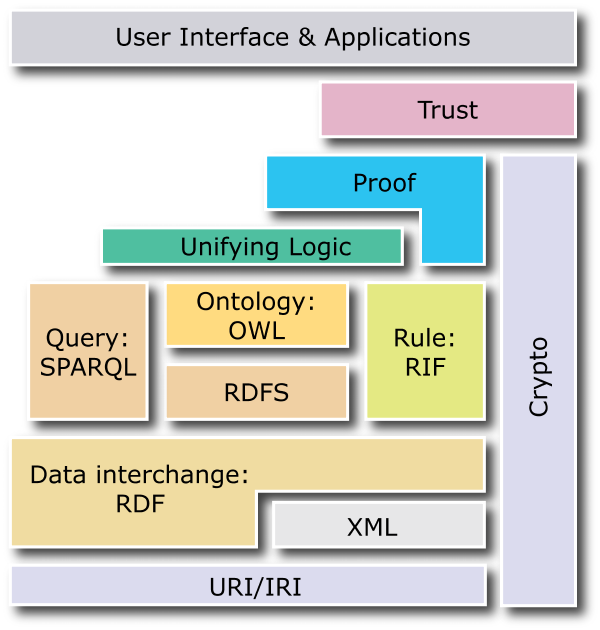
\includegraphics[width=0.7\linewidth]{chapters/background/img/layerCake.png}
\caption{The Semantic Web layer cake.}
\label{fig:swlayercake}
\end{figure}

\subsubsection{The Resource Description Framework (RDF)}

``The Resource Description Framework (RDF) is a framework for representing information in the Web.'' \cite{Klyne2004} It defines a standard model for representing and exchanging information on the Semantic Web. The RDF Specification has been a W3C Recommendation since 1999 \cite{Lassila1999}, with the latest version being a suite of six W3C Recommendations\footnote{\url{http://www.w3.org/standards/techs/rdf}}, published in 2004̇. 

\lstset{
	caption={RDF example represented in Turtle.}, 
	label=lst:rdfex,
	language=turtle
}
\setlength\parindent{0in}
\begin{minipage}[htb]{\linewidth}
\begin{lstlisting}
@prefix ex: <http://www.example.org/RDFexample#> .
@prefix rdf: <http://www.w3.org/1999/02/22-rdf-syntax-ns#> .
@prefix rdfs: <http://www.w3.org/2000/01/rdf-schema#> .
@prefix foaf: <http://xmlns.com/foaf/0.1/> .
@prefix bibo: <http://purl.org/ontology/bibo/> .
@prefix dcterms: <http://purl.org/dc/terms/> .

ex:doctorow a foaf:Person ;
   foaf:name "Cory Doctorow" ;
   foaf:firstName "Cory" ;
   foaf:surname "Doctorow" ;
   foaf:homepage <http://craphound.org> ;
   foaf:made ex:ftw .
ex:ftw a bibo:Book ;
   dcterms:title "For The Win" ;
   foaf:maker ex:doctorow ;
   bibo:issn13 "9780765322166" .
\end{lstlisting}
\end{minipage}
\setlength\parindent{0.21in}

RDF is designed to allow flexible representation of information. The underlying structure of any data represented with RDF is a graph, which is a collection of triples. Each triple represents an RDF statement, and is made up of a subject, a predicate (or property), and an object. An example is shown in Listing~\ref{lst:rdfex}. A triple can be seen as a graph made of two nodes, the subject and the object, connected through an arc, represented by the predicate. Thus, a set of triples can be represented as a graph by the corresponding set of nodes and arcs (see Figure~\ref{fig:rdfex} for an example). 
Any information about a resource can be expressed through triples, including information about a triple, through a process called reification. While a powerful feature, reification adds complexity, and is usually used sparsely. An extension to RDF allows statements to be grouped in \emph{named graphs} which helps avoid the use of reification to store meta-information about triples, like provenance for example.

\begin{figure}[th]
 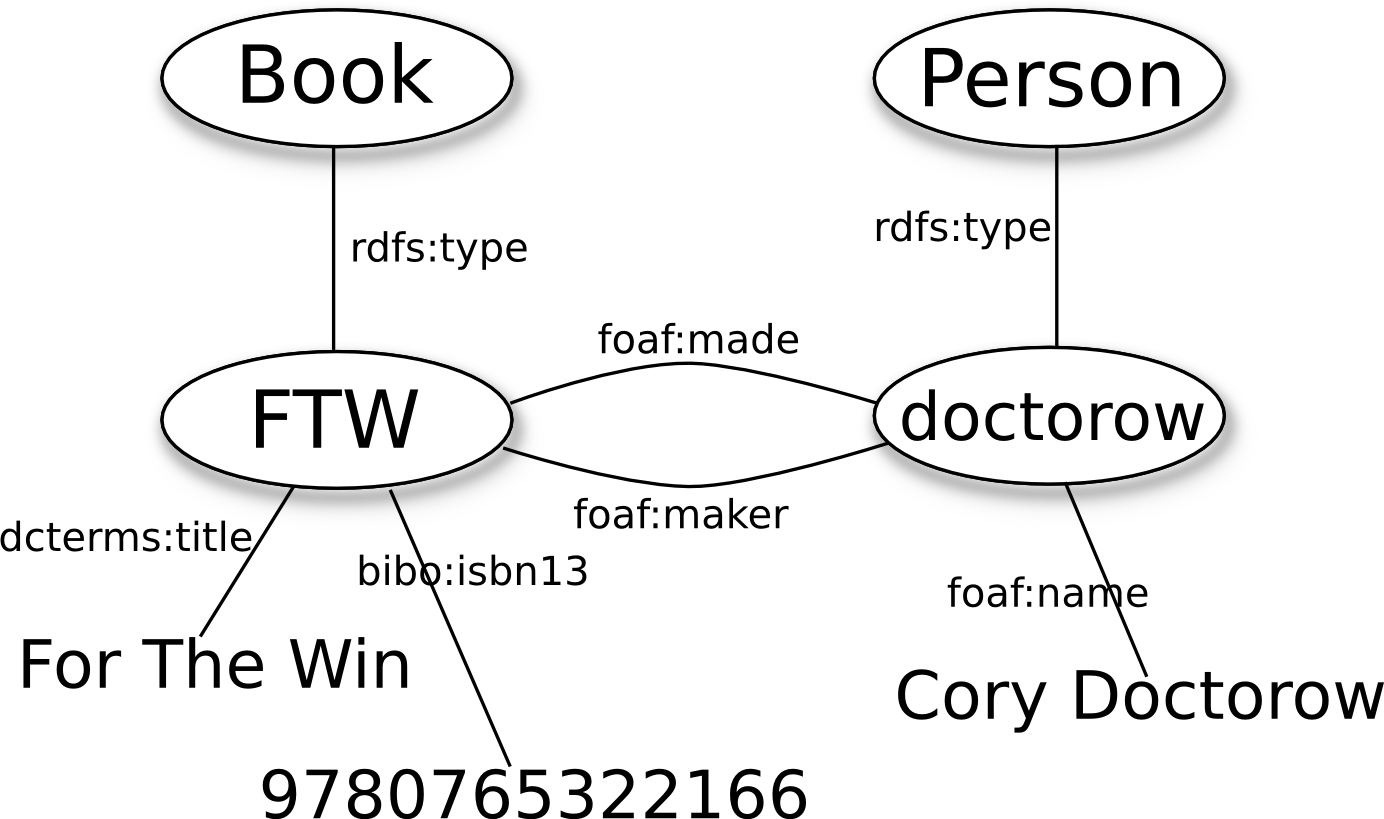
\includegraphics[width=0.8\linewidth]{chapters/background/img/rdfex}
\caption{RDF example represented as a graph.}
\label{fig:rdfex}
\end{figure} 

The RDF specification defines three types of elements: 
\begin{itemize}
 \item identified resources, which are represented by a URI. They can appear on any position in a triple.
 \item unidentified resources, called blank nodes, which cannot appear as predicates in triples. They are unnamed nodes within a graph, and using them can pose problems, thus it is discouraged \cite{Bizer2007}.
 \item literals, which can only appear as objects in a triple. Literals represent values of properties. They can be typed, using XML Schema datatypes, or can have a language tag.
\end{itemize}

RDF is a data model which can be serialised in several ways. The most popular serialisation of RDF was first RDF/XML \cite{Beckett2004}, due to the popularity and familiarity of XML. More recently however, other serialisations, more suitable for human consumption, have become preferred: N-Triples ~\cite{Grant2004}, Turtle \cite{Beckett2007}, and N3 \cite{BernersLee2006b}. RDFa \cite{Adida2008} is another syntax for RDF, which allows embedding of RDF statements in HTML pages. In the following chapters of the thesis, we will use the Turtle notation in listings.

SPARQL \cite{Prudhommeaux2008} is the recommended query language for RDF. Other query languages for RDF exist, including: 
\begin{itemize}
 \item RDF Query Language (RQL) \cite{Karvounarakis2002}, 
 \item Sesame RDF Query Language (SeRQL) \cite{Broekstra2003}, 
 \item RDF Data Query Language (RDQL) \cite{Seaborne2004}.
\end{itemize}

\subsubsection{Ontologies and Vocabularies}

RDF gives us the means to represent information in a unified way. However, this is not enough to make the information understandable to machines. Something more is needed, and that is a common, agreed-upon, and shared vocabulary to refer to things. This is represented by the ``Ontology'' layer in the SW layer cake. According to Gruber, an ontology is ``an explicit specification of'' [...] ``an abstract, simplified view of the world that we wish to represent for some purpose.'' \cite{Gruber1993}

RDF Schema (RDFS) \cite{Brickley2004} was created to support the use of RDF to define ontologies. The Web Ontology Language (OWL) is another formal language to define ontologies, which offers more expressive constructs than RDFS.

Both languages allow the definition of classes, hierarchies of classes, properties with domain and range, and hierarchies of properties. 

Ontologies can be: \emph{upper-level} (or top-level, or foundation) ontologies, defining high level, generic concepts, or \emph{domain} ontologies, which define concepts related to a specific, restricted domain.

Numerous vocabularies have emerged for the Semantic Web. Among them, a limited number have gained wide-spread adoption and recognition. The ones we use and refer to in this thesis are listed below:
\begin{itemize}
 \item Dublin Core Metadata Initiative (DCMI\footnote{\url{http://dublincore.org/}}) \cite{Nilsson2008} --- for ``core metadata for simple and generic resource descriptions'';
 \item Simple Knowledge Organization System (SKOS\footnote{\url{http://www.w3.org/2004/02/skos/}}) \cite{Miles2009} --- for sharing and linking data about ``knowledge organisation systems, such as thesauri, taxonomies, classification schemes and subject heading systems'';
 \item Friend Of A Friend (FOAF\footnote{\url{http://foaf-project.org}}) \cite{Brickley2005} --- for describing people and organisations;
 \item Semantically-Interlinked Online Communities (SIOC\footnote{\url{http://sioc-project.org}}) \cite{Breslin2005} --- for describing online communities; 
 \item Description Of A Project (DOAP\footnote{\url{https://github.com/edumbill/doap}}) --- for information about software projects;
 \item the Music Ontology (MO\footnote{\url{http://musicontology.com/}}) --- for ``describing music (i.e. artists, albums, tracks, but also performances, arrangements, etc.)'';
 \item GeoNames\footnote{\url{http://www.geonames.org/ontology/}} --- for geographic information.
\end{itemize}

\subsection{Linked Data}
\label{sec:ld}

The term Linked Data was first introduced by Berners-Lee in 2006 to define a set of best practices for publishing data on the Web \cite{BernersLee2006}. They became known as the ``Linked Data Principles'' and describe the recommended way to publish and connect data on the Web, so that ``it is machine readable, its meaning is explicitly described, it is linked to other external datasets and can in turn be linked from external datasets''.

In addition to these principles, the more recent Linking Open Data\footnote{\url{http://linkeddata.org}} project enables the creation of a huge amount of interlinked RDF data on the Web, from various open datasets, ranging from Health Care and Life Sciences (HCLS) information to the BBC programmes. 
